\documentclass[aspectratio=169]{beamer}

\usetheme{Madrid}
\usecolortheme{default}

% Remove navigation symbols
\setbeamertemplate{navigation symbols}{}
% Slide numbers (current only, no total)
\setbeamertemplate{footline}{%
  \hfill\insertframenumber\kern1em\vskip4pt%
}

\usepackage[T1]{fontenc}
\usepackage[utf8]{inputenc}
\usepackage{listings}
\usepackage{amsmath, amssymb, amsthm}
\usepackage{xcolor}
\usepackage{tikz}
\usetikzlibrary{arrows.meta, positioning}

% ---- Lean syntax highlighting (same colors as thesis) ----
\definecolor{keywordcolor}{rgb}{0.7, 0.1, 0.1}   % red
\definecolor{tacticcolor}{rgb}{0.0, 0.1, 0.6}     % blue
\definecolor{commentcolor}{rgb}{0.4, 0.4, 0.4}    % grey
\definecolor{symbolcolor}{rgb}{0.0, 0.1, 0.6}     % blue
\definecolor{sortcolor}{rgb}{0.1, 0.5, 0.1}       % green
\definecolor{attributecolor}{rgb}{0.7, 0.1, 0.1}  % red

\def\lstlanguagefiles{lstlean.tex}
\lstset{language=lean}

% ---- Math macros (same as thesis) ----
\newcommand{\E}{\mathbb{E}}
\renewcommand{\P}{\mathbb{P}}
\newcommand{\Q}{\mathbb{Q}}
\newcommand{\R}{\mathbb{R}}
\newcommand{\N}{\mathbb{N}}
\newcommand{\Var}{\mathbb{V}}

% ---- Lean code macro ----
\newcommand{\leancode}[1]{\textcolor{blue}{\nolinkurl{#1}}}

% ---- Title ----
\title{A Formally Verified Proof of Cram\'er's Theorem\\on Large Deviations}
\author{Kaan Berk Erdo\u{g}mu\c{s}}
\institute{University of Pennsylvania \\ Department of Mathematics \\ \vspace{0.3cm} \small Advisor: Prof. Henry Towsner}
\date{April 2026}

\begin{document}

%=================================================================
% TITLE
%=================================================================
\begin{frame}
  \titlepage
\end{frame}

%=================================================================
% OUTLINE
%=================================================================
\begin{frame}{Outline}
  \tableofcontents
\end{frame}

%=================================================================
\section{Introduction}
%=================================================================

\begin{frame}{What is Large Deviations Theory?}
  \begin{itemize}
    \item Study of the \textbf{asymptotic decay of tail probabilities}
    \item Let $X_1, X_2, \dots$ be i.i.d.\ random variables with mean $\mu = \E[X_1]$
    \item By the \textbf{Law of Large Numbers}: $\overline{X}_n \to \mu$ a.s.
    \item By the \textbf{Central Limit Theorem}: $\sqrt{n}(\overline{X}_n - \mu) \xrightarrow{d} \mathcal{N}(0, \sigma^2)$
  \end{itemize}
  \vspace{0.3cm}
  \begin{block}{Cram\'er's Theorem (1938) \cite{cramer1938sur}}
    For $a \ge \E[X_1]$, the tail probability decays \emph{exponentially}:
    \[
      \frac{1}{n}\log\P(\overline{X}_n \ge a) \;\to\; -I(a)
    \]
    where $\Lambda(t) = \log\E[e^{tX_1}]$ is the \textbf{cumulant generating function} (CGF) and $I(a) = \sup_{t \in \R}\{ta - \Lambda(t)\}$ is the \textbf{rate function} (Legendre transform of the CGF).
  \end{block}
\end{frame}

\begin{frame}{Why Formal Verification?}
  \begin{itemize}
    \item Cram\'er's Theorem's proof involves delicate arguments often glossed over:
      \begin{itemize}
        \item Limiting arguments in the lower bound proof
        \item Coercions between $\R$ and $\overline{\R}$ (e.g., $\log 0 = -\infty$)
        \item Precise enumeration of CLT preconditions under tilted measures
      \end{itemize}
      \vspace{0.3cm}
    \item Formal verification enforces \textbf{complete rigor}:
      \begin{itemize}
        \item Every assumption explicitly enumerated in the Lean type signature
        \item Machine-checked derivations --- no hand-waved steps
      \end{itemize}
  \end{itemize}
  \vspace{0.3cm}
  \begin{alertblock}{Novel Contribution}
    \textbf{First formalization of any large deviation result} in a proof assistant (using Lean 4 / Mathlib)
  \end{alertblock}
\end{frame}

\begin{frame}{In this Work}
  \begin{enumerate}
    \item A formal definition of the \textbf{Large Deviation Principle} (new Lean structure)
    \item Proof of the \textbf{upper bound} via the Chernoff bound (building on Mathlib)
    \item Proof of the \textbf{lower bound} via exponential tilting \& change of measure
    \item A precise \textbf{CLT assumption} under tilted measures, with informal justification
    \item The \textbf{final LDP result} combining both bounds
  \end{enumerate}
  % \vspace{0.3cm}
  % \begin{block}{Scale}
  %   \textbf{1,819 lines} of Lean 4 code across \textbf{5 files}, building on Mathlib's >2M-line library
  % \end{block}
\end{frame}

\begin{frame}{Code Structure}
  \begin{center}
    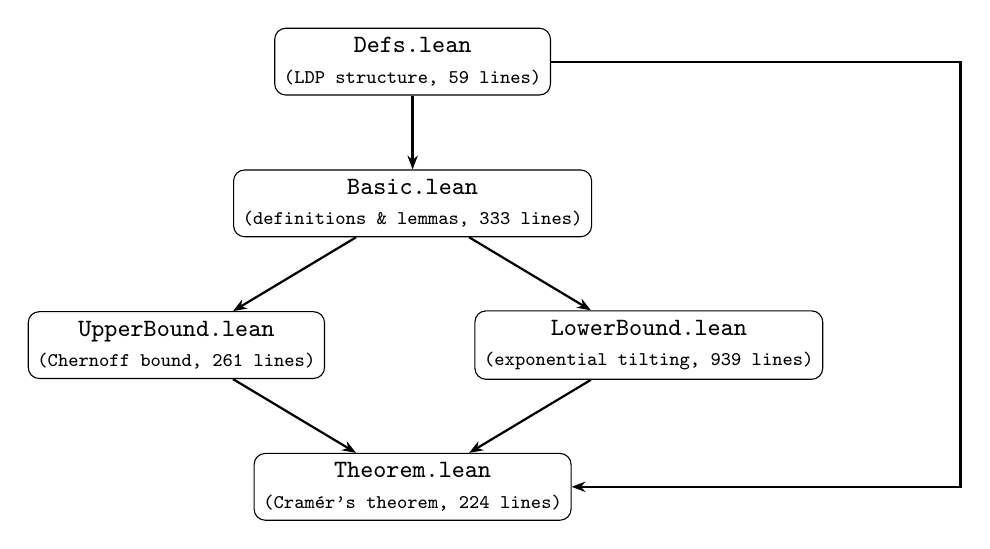
\begin{tikzpicture}[
        box/.style={draw, rounded corners, minimum width=3.2cm, minimum height=0.8cm,
        align=center, font=\small\ttfamily},
        arr/.style={-{Stealth[length=5pt]}, thick}
      ]
      \node[box] (defs)  at (0, 1.8)   {Defs.lean\\{\scriptsize(LDP structure, 59 lines)}};
      \node[box] (basic) at (0, 0)   {Basic.lean\\{\scriptsize(definitions \& lemmas, 333 lines)}};
      \node[box] (upper) at (-3,-1.8)  {UpperBound.lean\\{\scriptsize(Chernoff bound, 261 lines)}};
      \node[box] (lower) at (3, -1.8)  {LowerBound.lean\\{\scriptsize(exponential tilting, 939 lines)}};
      \node[box] (thm)   at (0, -3.6)  {Theorem.lean\\{\scriptsize(Cram\'er's theorem, 224 lines)}};

      \draw[arr] (defs)  -- (basic);
      \draw[arr] (basic) -- (upper);
      \draw[arr] (basic) -- (lower);
      \draw[arr] (upper) -- (thm);
      \draw[arr] (lower) -- (thm);
      % Route around the right side, wide enough to clear LowerBound
      \draw[arr] (defs.east) -- +(5.2,0) |- (thm.east);
    \end{tikzpicture}
  \end{center}
  \vspace{-0.1cm}
  \begin{center}
    \small Lower bound: $\approx$\textbf{half} of the total codebase
  \end{center}
\end{frame}

%=================================================================
\section{Related Work \& Context}
%=================================================================

\begin{frame}{Prior Formalizations of Probability}
  \begin{columns}[T]
    \begin{column}{0.5\textwidth}
      \textbf{Isabelle/HOL}
      \begin{itemize}
        \item H\"olzl \& Heller \cite{holzl2011}: measure theory, Lebesgue integral, Radon-Nikod\'ym, Fubini
        \item Avigad, H\"olzl, Serafin \cite{avigad2017clt}: \textbf{Central Limit Theorem}
        \item Hirata \cite{hirata2024levy}: L\'evy-Prokhorov metric
      \end{itemize}
      \vspace{0.3cm}
      \textbf{Rocq (Coq)}
      \begin{itemize}
        \item Affeldt \& Cohen \cite{affeldt2023}: measure \& integration theory
        \item Affeldt et al.\ \cite{affeldt2025concentration}: concentration inequalities, \textbf{Chernoff bound}
      \end{itemize}
    \end{column}
    \begin{column}{0.5\textwidth}
      \textbf{Lean 4 / Mathlib} \cite{mathlib2020}
      \begin{itemize}
        \item Ying \& Degenne \cite{ying2023martingale}: Doob's martingale convergence
        \item Degenne \cite{degenne2025kernels}: Markov kernels
        \item Sonoda et al.\ \cite{sonoda2025rademacher}: Rademacher complexity
        \item SLLN (Etemadi's proof \cite{etemadi1981slln}, in Mathlib)
        \item Marion, Zhu, Degenne \cite{marion2026clt}: \textbf{CLT} (merged March 2026)
      \end{itemize}
    \end{column}
  \end{columns}
\end{frame}

\begin{frame}{Our Contribution in Context}
  \begin{itemize}
    \item \textbf{No prior LDP formalization} in any proof assistant
      \begin{itemize}
        \item Not Cram\'er's theorem, Sanov's theorem, nor G\"artner-Ellis
        \item The LDP concept itself had not been formalized
      \end{itemize}
      \vspace{0.3cm}
    \item Closest prior work:
      \begin{itemize}
        \item Chernoff bounds in Rocq \cite{affeldt2025concentration} --- used in our upper bound
        \item CLT in Isabelle/HOL \cite{avigad2017clt}; recently Lean/Mathlib \cite{marion2026clt}
      \end{itemize}
      \vspace{0.3cm}
    \item We introduce the LDP as a \textbf{formal Lean structure}, prove Cram\'er's theorem,
      and account for the CLT gap
  \end{itemize}
\end{frame}

%=================================================================
\section{Setup \& Formalization}
%=================================================================

\begin{frame}{Setup \& Definitions}
  Let $(\Omega, \mathcal{F}, \P)$ be a probability space.
  Let $X_1, X_2, \dots$ be i.i.d.\ real-valued random variables.

  \begin{definition}[Partial Sums and Empirical Mean]
    \[
      S_n = \sum_{i=1}^{n} X_i, \qquad \overline{X}_n = \frac{S_n}{n}
    \]
  \end{definition}

  \begin{definition}[MGF, CGF, and Rate Function]
    \begin{align*}
      M_X(t) &= \E[e^{tX_1}] & &\text{(Moment Generating Function)} \\
      \Lambda(t) &= \log M_X(t) = \log \E[e^{tX_1}] & &\text{(Cumulant Generating Function)} \\
      I(x) &= \sup_{t \in \R}\{tx - \Lambda(t)\} & &\text{(Rate Function / Legendre Transform of $\Lambda(t)$)}
    \end{align*}
  \end{definition}
  Since $t=0$ yields $0 \cdot x - \Lambda(0) = 0$, we have $I(x) \ge 0$ for all $x$.
\end{frame}

\begin{frame}{The Large Deviation Principle}
  \begin{definition}[LDP --- General Form {\cite{dembo1998large}}]
    A sequence $Z_n$ satisfies an \textbf{LDP} with rate function $I$ if for all $A$:
    \[
      -\inf_{x \in \mathring{A}} I(x) \;\le\; \liminf_{n\to\infty} \frac{1}{n}\log\P(Z_n \in A) \;\le\; \limsup_{n\to\infty} \frac{1}{n}\log\P(Z_n \in A) \;\le\; -\inf_{x \in \overline{A}} I(x)
    \]
  \end{definition}

  \begin{block}{Specialization to upper tail sets $[a,\infty)$}
    Both bounds collapse to the same rate function $I(a)$:
    \begin{align*}
      \text{Upper:}\quad & \limsup_{n\to\infty} \frac{1}{n}\log\P(\overline{X}_n \ge a) \le -I(a) \\
      \text{Lower:}\quad & \liminf_{n\to\infty} \frac{1}{n}\log\P(\overline{X}_n \ge a) \ge -I(a)
    \end{align*}
  \end{block}
\end{frame}

\begin{frame}{Tilted Measure}
  \begin{definition}[Tilted Measure]
    For a tilting parameter $t \in \R$, define $\Q_{n,t}$ via the Radon-Nikodym derivative:
    \[
      \frac{d\Q_{n,t}}{d\P} = \frac{e^{tS_n}}{\E_\P[e^{tS_n}]} = \frac{e^{tS_n}}{(M_X(t))^n} = e^{tS_n - n\Lambda(t)}
    \]
  \end{definition}
  \vspace{0.2cm}
  We will show that:
  \begin{itemize}
    \item Reweights probability to make $\{\overline{X}_n \ge a\}$ a \textbf{typical event}
    \item Key tool for the \textbf{lower bound}: transforms rare event $\to$ typical event
    \item Under $\Q_{n,t}$: $\E_{\Q_{n,t}}[\overline{X}_n] = \Lambda'(t)$
    \item Pick $t$ so that $\Lambda'(t) = a$ $\implies$ mean shifts to $a$
  \end{itemize}
\end{frame}

\begin{frame}{Case $a < \E[X_1]$: Not a Rare Event}
  \begin{itemize}
    \item When $a < \E[X_1]$, $\{\overline{X}_n \ge a\}$ is \textbf{not} a rare event
    \item By the \textbf{Strong Law of Large Numbers}:
      \[
        \overline{X}_n \to \E[X_1] \;\text{a.s.} \quad \implies \quad \P(\overline{X}_n \ge a) \to 1
      \]
    \item Define $I(a) = 0$ in this case; LDP bounds hold trivially:
      \begin{itemize}
        \item Upper: $\P(\overline{X}_n \ge a) \le 1 \implies \frac{1}{n}\log\P \le 0 = -I(a)$
        \item Lower: $\P(\overline{X}_n \ge a) \to 1 \implies \frac{1}{n}\log\P \to 0 = -I(a)$
      \end{itemize}
  \end{itemize}
  \vspace{0.2cm}
  \begin{block}{Effective Rate Function}
    \[
      I(a) =
      \begin{cases}
        \sup_{t \in \R}\{ta - \Lambda(t)\} & \text{if } a \ge \E[X_1] \\
        0 & \text{if } a < \E[X_1]
      \end{cases}
    \]
  \end{block}
\end{frame}

%=================================================================
% Formalization Framework (part of Setup & Formalization)
%=================================================================

\begin{frame}{Lean 4 \& Type Theory}
  \begin{itemize}
    \item \textbf{Lean 4} \cite{demoura2021lean4}: programming language and proof assistant. Code that type-checks is provably correct.
    \item \textbf{Mathlib} \cite{mathlib2020}: community math library (>2M lines), providing Real Analysis, Measure Theory, and Probability Foundations:
      $\sigma$-algebras, probability measures, MGF/CGF, tilted measures, SLLN
      \vspace{0.2cm}
    \item Built on \textbf{dependent type theory}, not set theory
      \begin{itemize}
        \item E.g. $\R$ and $\overline{\R}$ (\leancode{EReal}) are distinct types:
          \begin{itemize}
            \item $x \in \R$ is \textbf{not} implicitly an element of $\overline{\R}$
            \item Requires explicit coercions $\uparrow\! x$, introduces overhead to formalization
          \end{itemize}
      \end{itemize}
  \end{itemize}
\end{frame}

\begin{frame}[fragile]{Basic Lean Syntax}
  \begin{itemize}
    \item \textbf{Arguments:}
      \begin{itemize}
        \item \leancode{ {x} } -- implicit (inferred by the type checker)
        \item \leancode{(x)} -- explicit (supplied by the caller)
        \item \leancode{[instance]} -- type class instance
      \end{itemize}
      \vspace{0.2cm}
    \item \leancode{noncomputable} -- definition involves non-constructive axioms;\\
      not compilable to executable code, but fully type-checked and verified
      \vspace{0.2cm}
    \item \textbf{Filters} -- unified framework for limits and asymptotics:
      \begin{itemize}
        \item $\forall^\text{f}\, n\;\text{in}\;\text{atTop}$ = ``for all sufficiently large $n$''
        \item \leancode{limsup} and \leancode{liminf} defined via filters
        \item $\textcolor{blue}{\text{Tendsto}}~f~\textcolor{blue}{\text{atTop}} (\mathcal{N}~c)$ = ``$f(n) \to c$''
      \end{itemize}
  \end{itemize}
\end{frame}

\begin{frame}[fragile]{Formal Definitions (Lean)}
\begin{lstlisting}[basicstyle=\ttfamily\scriptsize]
variable {Ω : Type*} [MeasureSpace Ω]
variable (X : ℕ → Ω → ℝ)

/-- The partial sum X_0 + ... + X_{n-1}. -/
noncomputable def partialSum (n : ℕ) : Ω → ℝ :=  ∑ i ∈ Finset.range n, X i

/-- The empirical mean Sₙ / n. -/
noncomputable def empiricalMean (n : ℕ) : Ω → ℝ := fun ω => partialSum X n ω / n

/-- Rate function: Legendre transform of the CGF. -/
noncomputable def I (x : ℝ) : ℝ := ⨆ t : ℝ, t * x - cgf (X 0) ℙ t

/-- Effective rate function for the LDP statement. -/
noncomputable def upperTailRateFunction (a : ℝ) : ℝ :=
  if 𝔼[X 0] ≤ a then I X a else 0

/-- The exponentially tilted measure, tilted by t · Sₙ. -/
noncomputable def ℚₙₜ (μ : Measure Ω) (n : ℕ) (t : ℝ) :
    Measure Ω :=  Measure.tilted μ (fun ω => t * partialSum X n ω)
\end{lstlisting}
  {\small\textit{Note:} $\bigsqcup$ is notation for the indexed supremum (\leancode{iSup}); Lean indexes from 0, so \leancode{X} \leancode{0} corresponds to $X_1$}
\end{frame}

\begin{frame}[fragile]{The Large Deviation Principle (Lean)}
\begin{lstlisting}[basicstyle=\ttfamily\scriptsize]
structure LargeDeviationPrinciple
    (Y : ℕ → Ω → ℝ) (I : ℝ → ℝ) : Prop where
  upperBound : ∀ a : ℝ,
    limsup (fun n : ℕ => ((1 : ℝ) / (n : ℝ) : EReal) * ENNReal.log (ℙ {ω | Y n ω ≥ a})) atTop
      ≤ (- I a : EReal)
  lowerBound : ∀ a : ℝ,
    (- I a : EReal) ≤
      liminf (fun n : ℕ => ((1 : ℝ) / (n : ℝ) : EReal) * ENNReal.log (ℙ {ω | Y n ω ≥ a})) atTop
\end{lstlisting}
  \vspace{0.2cm}
  \begin{itemize}
    \item Uses \leancode{EReal} to handle $\log 0 = -\infty$ and \leancode{ENNReal.log}: $[0, \infty] \to [-\infty, \infty]$
    \item Separated upper/lower bounds for independent proofs
  \end{itemize}
\end{frame}

%=================================================================
\section{Assumptions \& Theorem Statement}
%=================================================================

\begin{frame}[fragile]{Assumptions (Part 1)}
  \begin{itemize}
    \item \textbf{Measurability:} $X_i$ are measurable
\begin{lstlisting}[basicstyle=\ttfamily\scriptsize]
variable (h_meas : ∀ n, Measurable (X n))
\end{lstlisting}
    \item \textbf{Independence:} $X_i$ are mutually independent
\begin{lstlisting}[basicstyle=\ttfamily\scriptsize]
variable (h_indep : iIndepFun X ℙ)
\end{lstlisting}
    \item \textbf{Identically Distributed:} same distribution as $X_0$
\begin{lstlisting}[basicstyle=\ttfamily\scriptsize]
variable (h_ident : ∀ n, IdentDistrib (X n) (X 0) ℙ ℙ)
\end{lstlisting}
    \item \textbf{Integrability:} $X_1$ measurable and $\E[|X_1|] < \infty$
\begin{lstlisting}[basicstyle=\ttfamily\scriptsize]
variable (h_int : Integrable (X 0) ℙ)
\end{lstlisting}
    \item \textbf{Finite MGF:} $\E[e^{tX_1}] < \infty$ for all $t \in \R$
\begin{lstlisting}[basicstyle=\ttfamily\scriptsize]
variable (h_mgf : ∀ t : ℝ,
  Integrable (fun ω => Real.exp (t * X 0 ω)) ℙ)
\end{lstlisting}
  \end{itemize}
\end{frame}

\begin{frame}[fragile]{Assumptions (Part 2)}
  \begin{itemize}
    \item \textbf{Bounded rate function:} $\{ta - \Lambda(t)\}$ is bounded above
\begin{lstlisting}[basicstyle=\ttfamily\scriptsize]
variable (h_bdd : ∀ a : ℝ,
  BddAbove (Set.range (fun t => t * a - cgf (X 0) ℙ t)))
\end{lstlisting}
    \item \textbf{Non-degeneracy:} $\Lambda''(t) > 0$ for all $t$
\begin{lstlisting}[basicstyle=\ttfamily\scriptsize]
variable (h_non_deg : ∀ t : ℝ,
  0 < iteratedDeriv 2 (cgf (X 0) ℙ) t)
\end{lstlisting}
    \item \textbf{Exposed points:} $\forall a \ge \E[X], \exists t: \Lambda'(t) = a$
\begin{lstlisting}[basicstyle=\ttfamily\scriptsize]
variable (h_exposed : ∀ a : ℝ, 𝔼[X 0] ≤ a →
  ∃ t, deriv (cgf (X 0) ℙ) t = a)
\end{lstlisting}
  \end{itemize}
\end{frame}

\begin{frame}[fragile]{Assumptions (Part 3): CLT under Tilted Measures}
  \begin{itemize}
    \item \textbf{CLT under tilted measures:} For $\Lambda'(t) = a$, under the tilted measure $\Q_{n,t}$, the sample mean concentrates around $a$:
      $$\forall \delta > 0,\; \forall \varepsilon > 0,\quad \Q_{n,t}\!\left(\overline{X}_n \in [a,\, a+\delta]\right) \geq \tfrac{1}{2} - \varepsilon \quad \text{eventually}$$
  \end{itemize}
\begin{lstlisting}[basicstyle=\ttfamily\scriptsize]
variable (h_clt_axiom :
    iIndepFun X ℙ →
    (∀ n, IdentDistrib (X n) (X 0) ℙ ℙ) →
    (∀ n, Measurable (X n)) →
    Integrable (X 0) ℙ →
    (∀ t : ℝ, Integrable (fun ω => Real.exp (t * X 0 ω)) ℙ) →
    (∀ t : ℝ, 0 < iteratedDeriv 2 (cgf (X 0) ℙ) t) →
    ∀ (t a : ℝ), ∀ δ > 0, ∀ ε > 0,
    deriv (cgf (X 0) ℙ) t = a →
      ∀ᶠ n in atTop,
      (1 / 2 - ε : ℝ) ≤
        ((Measure.tilted ℙ
          (fun ω => t * (∑ i ∈ Finset.range n, X i ω)))
          {ω | (∑ i ∈ Finset.range n, X i ω) / n
            ∈ Set.Icc a (a + δ)}).toReal)
\end{lstlisting}
\end{frame}

%=================================================================
% Theorem Statement (part of Assumptions & Theorem Statement)
%=================================================================

\begin{frame}[fragile]{Cram\'er's Theorem --- Formal Statement}
  \begin{theorem}[Cram\'er's Theorem]
    The empirical means $\overline{X}_n$ satisfy an LDP with rate function
    \leancode{upperTailRateFunction}:
    \begin{itemize}
      \item For $a \ge \E[X]$: rate function $I(a) = \sup_t\{ta - \Lambda(t)\}$
      \item For $a < \E[X]$: rate function $0$ (trivial case via SLLN)
    \end{itemize}
  \end{theorem}
  \vspace{0.2cm}
\begin{lstlisting}[basicstyle=\ttfamily\scriptsize]
include h_indep h_meas h_ident h_mgf h_int h_bdd h_non_deg h_exposed h_clt_axiom in
/-- **Cramér's Theorem**: For i.i.d. random variables
with finite MGF, the empirical mean satisfies a large
deviation principle with rate function given by the
Legendre transform of the CGF. -/
theorem cramers_theorem : LargeDeviationPrinciple  (empiricalMean X) (upperTailRateFunction X)
\end{lstlisting}
  \begin{center}
    \small Verified by Lean's type-theoretic kernel
  \end{center}
\end{frame}

%=================================================================
% Basic Properties (part of Upper Bound section)
%=================================================================

\begin{frame}[fragile]{Basic Lemmas}
  \begin{enumerate}
    \item \textbf{Finite MGF of identically distributed variables:} $\E[e^{tX_i}] < \infty$ for all $i$, $t$
\begin{lstlisting}[basicstyle=\ttfamily\tiny]
lemma integrable_exp_of_identDistrib (i : ℕ) (t : ℝ) : Integrable (fun ω => Real.exp (t * X i ω)) ℙ
\end{lstlisting}
    \item \textbf{Measurability of partial sum $S_n$:}
\begin{lstlisting}[basicstyle=\ttfamily\tiny]
lemma measurable_partialSum (n : ℕ) : Measurable (partialSum X n)
\end{lstlisting}
    \item \textbf{Measurability of empirical mean $\overline{X}_n$:}
\begin{lstlisting}[basicstyle=\ttfamily\tiny]
lemma measurable_empiricalMean (n : ℕ) : Measurable (empiricalMean X n)
\end{lstlisting}
    \item \textbf{Interior of integrable exponential set:} $\forall t \in \R,\; t \in \textnormal{int}\{t \mid \E[e^{tX_1}] < \infty\}$
\begin{lstlisting}[basicstyle=\ttfamily\tiny]
lemma mem_interior_integrableExpSet (t : ℝ) :
    t ∈ interior (integrableExpSet (X 0) ℙ)
\end{lstlisting}
  \end{enumerate}
\end{frame}

\begin{frame}[fragile]{Basic Lemmas (Part 2)}
  \begin{enumerate}\setcounter{enumi}{4}
    \item \textbf{CGF lower bound:} $\Lambda(t) \ge t\E[X]$ \quad (Jensen's inequality)
\begin{lstlisting}[basicstyle=\ttfamily\tiny]
lemma cgf_ge_mul_expect {Y : Ω → ℝ} (h_int : Integrable Y ℙ)
    (h_mgf : ∀ t : ℝ, Integrable (fun ω => Real.exp (t * Y ω)) ℙ) (t : ℝ) :
    cgf Y ℙ t ≥ t * 𝔼[Y]
\end{lstlisting}
    \item \textbf{Rate function negative for negative parameter:} if $t < 0$ and $a \ge \E[X]$: $ta - \Lambda(t) \le 0$
\begin{lstlisting}[basicstyle=\ttfamily\tiny]
lemma rate_function_neg_param_le_zero {Y : Ω → ℝ} (h_int : Integrable Y ℙ)
    (h_mgf : ∀ t : ℝ, Integrable (fun ω => Real.exp (t * Y ω)) ℙ)
    {t a : ℝ} (ht : t < 0) (ha : 𝔼[Y] ≤ a) : t * a - cgf Y ℙ t ≤ 0
\end{lstlisting}
    \item \textbf{Finite MGF of partial sum $S_n$:}
\begin{lstlisting}[basicstyle=\ttfamily\tiny]
lemma integrable_exp_sum (t : ℝ) (n : ℕ) :
    Integrable (fun ω => Real.exp (t * partialSum X n ω)) ℙ
\end{lstlisting}
    \item \textbf{Tilted measure is a probability measure:} $\Q_{n,t}(\Omega) = 1$
\begin{lstlisting}[basicstyle=\ttfamily\tiny]
lemma isProbabilityMeasure_tilted_partialSum (t : ℝ) (n : ℕ) : IsProbabilityMeasure (ℚₙₜ X ℙ n t)
\end{lstlisting}
  \end{enumerate}
\end{frame}

\begin{frame}[fragile]{Basic Lemmas (Part 3)}
  \begin{enumerate}\setcounter{enumi}{8}
    \item \textbf{Interior of integrable exp.\ set of partial sums:}
\begin{lstlisting}[basicstyle=\ttfamily\tiny]
lemma mem_interior_integrableExpSet_partialSum (t : ℝ) (n : ℕ) :
    t ∈ interior (integrableExpSet (partialSum X n) ℙ)
\end{lstlisting}
    \item \textbf{Rate function supremum at non-negative $t$:} $I(a) = \sup_{t \ge 0}\{ta - \Lambda(t)\}$ for $a \ge \E[X]$
\begin{lstlisting}[basicstyle=\ttfamily\tiny]
lemma rateFunction_eq_sup_nonneg (a : ℝ) (h_mean : 𝔼[X 0] ≤ a) :
    I X a = ⨆ t : {(x : ℝ) | 0 ≤ x}, (t : ℝ) * a - cgf (X 0) ℙ t
\end{lstlisting}
    \item \textbf{MGF of partial sum:} $M_{S_n}(t) = e^{n\Lambda(t)}$
\begin{lstlisting}[basicstyle=\ttfamily\tiny]
lemma mgf_sum_eq_exp_n_prod_cgf (n : ℕ) (t : ℝ) :
    mgf (partialSum X n) ℙ t = Real.exp (n * cgf (X 0) ℙ t)
\end{lstlisting}
    \item \textbf{CGF of partial sum:} $\Lambda_{S_n}(t) = n\Lambda(t)$
\begin{lstlisting}[basicstyle=\ttfamily\tiny]
lemma cgf_sum_eq_n_prod_cgf (n : ℕ) (t : ℝ) :
    cgf (partialSum X n) ℙ t = (n : ℝ) * cgf (X 0) ℙ t
\end{lstlisting}
  \end{enumerate}
\end{frame}

%=================================================================
\section{Upper Bound: The Chernoff Bound}
%=================================================================

\begin{frame}{Upper Bound Strategy}
  \begin{block}{Goal}
    \[
      \limsup_{n \to \infty} \frac{1}{n}\log\P(\overline{X}_n \ge a) \le -I(a)
    \]
  \end{block}
  \vspace{0.3cm}
  \textbf{Approach:} Exponential Markov's inequality (= Chernoff bound)
  \begin{enumerate}
    \item Apply Markov's inequality to $e^{tS_n}$
    \item Factor the expectation using independence
    \item Take logarithms and optimize over $t \ge 0$
    \item Show the supremum over $t \ge 0$ equals $I(a)$
  \end{enumerate}
\end{frame}

\begin{frame}{Chernoff Bound Derivation}
  Since $x \mapsto e^{tx}$ is monotonically increasing, apply Markov's inequality:
  \[
    \P(\overline{X}_n \ge a) = \P(e^{tS_n} \ge e^{tna}) \le e^{-tna}\E[e^{tS_n}]
  \]

  By independence, the expectation factors:
  \[
    \E[e^{tS_n}] = \prod_{i=1}^n \E[e^{tX_i}] = \left(\E[e^{tX_1}]\right)^n = e^{n\Lambda(t)}
  \]

  Therefore:
  \begin{equation*}
    \boxed{\P(\overline{X}_n \ge a) \le e^{-n(ta - \Lambda(t))}}
  \end{equation*}
\end{frame}

\begin{frame}{From Chernoff to Rate Function}
  Taking $\frac{1}{n}\log$:
  \[
    \frac{1}{n}\log\P(\overline{X}_n \ge a) \le -(ta - \Lambda(t))
  \]

  The bound is \textbf{independent of $n$}, so taking $\limsup$ preserves it.

  \vspace{0.3cm}
  Optimizing over $t \ge 0$:
  \[
    \limsup_{n\to\infty} \frac{1}{n}\log\P(\overline{X}_n \ge a) \le -\sup_{t \ge 0}\{ta - \Lambda(t)\}
  \]

  \vspace{0.2cm}
  \begin{block}{Key identity}
    $\sup_{t \ge 0}\{ta - \Lambda(t)\} = \sup_{t \in \R}\{ta - \Lambda(t)\} = I(a)$

    \smallskip
    \textit{Proof:} If $t < 0$ and $a \ge \E[X]$, then $ta - \Lambda(t) \le 0$ by Jensen's inequality ($\Lambda(t) \ge t\E[X]$). Since $t \cdot 0 - \Lambda(0) = 0$ negative $t$ cannot improve the supremum.
  \end{block}
\end{frame}

\begin{frame}{Worked Example: Exponential Distribution}
  Let $X_i \sim \text{Exp}(\lambda)$ with $\E[X_1] = 1/\lambda$.

  \begin{columns}[T]
    \begin{column}{0.5\textwidth}
      \textbf{CGF:}
      \[
        \Lambda(t) = \log\lambda - \log(\lambda - t), \; t < \lambda
      \]

      \textbf{Rate function:}
      Optimize $g(t) = ta - \Lambda(t)$:
      \[
        g'(t) = 0 \implies t^* = \lambda - \tfrac{1}{a}
      \]
      \[
        I(a) = \lambda a - 1 - \log(\lambda a)
      \]
    \end{column}
    \begin{column}{0.5\textwidth}
      \textbf{Sanity check:}
      \begin{itemize}
        \item At $a = 1/\lambda$ (the mean):
          \[
            I(1/\lambda) = 1 - 1 - \log 1 = 0 \;\checkmark
          \]
        \item As $a$ increases: $I(a) > 0$
        \item Exponential decay of tail confirmed
      \end{itemize}
      \vspace{0.3cm}
      \textbf{Upper bound:}
      \[
        \limsup \frac{1}{n}\log\P(\overline{X}_n \ge a) \le -I(a)
      \]
    \end{column}
  \end{columns}
\end{frame}

\begin{frame}[fragile]{Formalized Upper Bound (Lean)}
  \textbf{Chernoff bound lemma:}
\begin{lstlisting}[basicstyle=\ttfamily\scriptsize]
lemma prob_mean_ge_le_exp (t a : ℝ) (ht : 0 ≤ t)
    (n : ℕ) (hn_pos : 0 < n) :
    (ℙ {ω | empiricalMean X n ω ≥ a}).toReal
      ≤ Real.exp (-(n : ℝ) * (t * a - cgf (X 0) ℙ t))
\end{lstlisting}
  \vspace{0.2cm}
  \textbf{Upper bound theorem:}
\begin{lstlisting}[basicstyle=\ttfamily\scriptsize]
theorem cramer_upper_bound (a : ℝ) (h_mean : 𝔼[X 0] ≤ a) :
    limsup (fun n : ℕ =>
      ((1 : ℝ) / (n : ℝ) : EReal) *
        ENNReal.log (ℙ {ω | empiricalMean X n ω ≥ a}))
      atTop ≤ (- I X a : EReal)
\end{lstlisting}
  \vspace{0.2cm}
  \begin{itemize}
    \item Several \textbf{EReal coercion lemmas} needed to lift $\R$ results to $\overline{\R}$
    \item Infimum of negations, coercion of infima, etc.
  \end{itemize}
\end{frame}

%=================================================================
\section{Lower Bound: Exponential Tilting}
%=================================================================

\begin{frame}{Lower Bound Strategy}
  \begin{block}{Goal}
    \[
      \liminf_{n \to \infty} \frac{1}{n}\log\P(\overline{X}_n \ge a) \ge -I(a)
    \]
  \end{block}
  \vspace{0.3cm}
  \textbf{Approach:} Change of measure to tilted $\Q_{n,t}$
  \begin{enumerate}
    \item Restrict to a concentrated set $E_n = \{\overline{X}_n \in [a, a+\delta]\}$
    \item Change of measure: bound $\P(E_n)$ from below using $\Q_{n,t}(E_n)$
    \item Use CLT to show $\Q_{n,t}(E_n)$ is bounded away from 0
    \item Take limits and send $\delta \to 0$
  \end{enumerate}
  \vspace{0.2cm}
  \begin{center}
    \textbf{Key idea:} Tilting transforms the rare event into a typical one
  \end{center}
\end{frame}

\begin{frame}{Why Tilting Works}
  Rearranging the Radon-Nikodym derivative:
  \[
    d\P = e^{-n(t\overline{X}_n - \Lambda(t))}\,d\Q_{n,t}
  \]

  This \textbf{matches} the Chernoff bound $\P(\overline{X}_n \ge a) \le e^{-n(ta - \Lambda(t))}$,
  except $\overline{X}_n$ replaces $a$.

  \vspace{0.3cm}
  If we could show $\overline{X}_n \approx a$ under $\Q_{n,t}$, the bound becomes tight!

  \vspace{0.3cm}
  \begin{block}{Mean and Variance under $\Q_{n,t}$}
    \begin{align*}
      \E_{\Q_{n,t}}[\overline{X}_n] &= \Lambda'(t) \quad\quad \text{(pick $t$ so $\Lambda'(t) = a$)} \\
      \Var_{\Q_{n,t}}(\overline{X}_n) &= \frac{\Lambda''(t)}{n} \to 0
    \end{align*}
    Tilted measure \textbf{re-centers} at $a$ with \textbf{shrinking variance}
  \end{block}
\end{frame}

\begin{frame}{CLT under Tilted Measures}
  Define standardized variables:
  \[
    Y_i = \frac{X_i - \Lambda'(t)}{\sqrt{\Lambda''(t)}}, \qquad Z_n = \frac{1}{\sqrt{n}}\sum_{i=1}^n Y_i
  \]

  \textbf{Key computation:} The characteristic function of $Y_i$ under $\Q_{n,t}$ is
  \[
    \varphi_{Y_i, \Q_{n,t}}(\theta) = \boxed{e^{-\Lambda(t)}\E_\P[e^{i\theta Y_i + tX_i}]}
  \]
  which is \textbf{independent of $n$}. Therefore:
  \[
    \varphi_{Z_n, \Q_{n,t}}(\theta)
    = \left(\varphi_{Y_1, \Q_{n,t}}\!\left(\frac{\theta}{\sqrt{n}}\right)\right)^{\!n}
    \xrightarrow{n\to\infty} e^{-\theta^2/2}
  \]

  By \textbf{L\'evy's Continuity Theorem}: $Z_n \xrightarrow{d} \mathcal{N}(0,1)$ under $\Q_{n,t}$.
\end{frame}

\begin{frame}[fragile]{CLT Corollary (the assumption)}
  \begin{corollary}
    For any $\delta > 0$:
    \[
      \Q_{n,t}(\overline{X}_n \in [a, a+\delta]) \;\to\; \frac{1}{2}
    \]
  \end{corollary}

  \vspace{0.1cm}
  \textit{Proof sketch:} The event $\overline{X}_n \in [a, a+\delta]$ is equivalent to $Z_n \in [0, \delta\sqrt{n/\Lambda''(t)}]$. As the upper bound $\to \infty$, the probability converges to $1/2$ by the standard normal CDF: $\Phi(\infty) - \Phi(0) = 1/2$.

  \vspace{0.3cm}
  Formalized as \leancode{h\_clt\_axiom}:
  \begin{itemize}
    \item All preconditions explicitly listed for future replacement
    \item Once Mathlib CLT is adapted to tilted measures, this axiom can be directly replaced
  \end{itemize}
\end{frame}

\begin{frame}{Lower Bound Proof}
  Restrict to $E_n = \{\overline{X}_n \in [a, a+\delta]\}$.

  \textbf{Step 1:} Change of measure
  \[
    \P(\overline{X}_n \ge a) \ge \P(E_n) \ge e^{-n(t(a+\delta) - \Lambda(t))}\,\Q_{n,t}(E_n)
  \]

  \textbf{Step 2:} Take scaled logarithms
  \[
    \frac{1}{n}\log\P(\overline{X}_n \ge a) \ge -(ta - \Lambda(t)) - t\delta + \frac{1}{n}\log\Q_{n,t}(E_n)
  \]

  \textbf{Step 3:} CLT gives $\Q_{n,t}(E_n) \ge c > 0$, so $\frac{1}{n}\log\Q_{n,t}(E_n) \to 0$

  \textbf{Step 4:} Send $\delta \to 0$:
  \[
    \liminf_{n\to\infty} \frac{1}{n}\log\P(\overline{X}_n \ge a) \ge -(ta - \Lambda(t))
  \]

  \textbf{Step 5:} Identify $I(a) = ta - \Lambda(t)$ (unique maximizer since $\Lambda$ strictly convex)
\end{frame}

\begin{frame}{Worked Example: Exponential Distribution (Lower Bound)}
  \textbf{Tilted distribution:} Under $\Q_{n,t^*}$ with $t^* = \lambda - 1/a$:
  \[
    e^{t^* x} \cdot \lambda e^{-\lambda x} \propto e^{-x/a} \quad\implies\quad X_i \sim \text{Exp}(1/a)
  \]
  The exponential family is \textbf{closed under tilting}.

  \vspace{0.3cm}
  \textbf{Shifted mean:} $\E_{\Q_{n,t^*}}[X_i] = a$ --- rare event becomes typical!

  \vspace{0.2cm}
  \textbf{Lower bound:}
  \[
    \liminf_{n\to\infty} \frac{1}{n}\log\P(\overline{X}_n \ge a) \ge -I(a) = -(\lambda a - 1 - \log(\lambda a))
  \]

  \vspace{0.2cm}
  \textbf{Matching the upper bound} $\implies$ the LDP is tight:
  \[
    \lim_{n\to\infty} \frac{1}{n}\log\P(\overline{X}_n \ge a) = -I(a) \qquad\checkmark
  \]
\end{frame}

\begin{frame}[fragile]{Formalized Lower Bound (Lean)}
  \textbf{Change of measure:} For $E = \{\overline{X}_n \in [a, a+\delta]\}$ and $t > 0$:
  $\P(E) \ge e^{-n(t(a+\delta) - \Lambda(t))}\, \Q_{n,t}(E)$
\begin{lstlisting}[basicstyle=\ttfamily\scriptsize]
lemma change_of_measure_lower_bound (a δ t : ℝ)
    (n : ℕ) (_hδ : 0 < δ) (ht : 0 < t) ... :
    let E := {ω | empiricalMean X n ω ∈ Set.Icc a (a + δ)}
    (ℙ E).toReal ≥
      Real.exp (-n * (t * (a + δ) - cgf (X 0) ℙ t)) * ((ℚₙₜ X ℙ n t) E).toReal
\end{lstlisting}
  \vspace{0.2cm}
  \textbf{Lower bound theorem:} For $a \ge \E[X]$: \;$\liminf_{n\to\infty} \frac{1}{n}\log\P(\overline{X}_n \ge a) \ge -I(a)$
\begin{lstlisting}[basicstyle=\ttfamily\scriptsize]
theorem cramer_lower_bound (a : ℝ) (h_mean : 𝔼[X 0] ≤ a) :
    (- I X a : EReal) ≤
      liminf (fun n : ℕ => ((1 : ℝ) / (n : ℝ) : EReal)
                           * ENNReal.log (ℙ {ω | empiricalMean X n ω ≥ a})) atTop
\end{lstlisting}
  \vspace{0.2cm}
  \begin{center}
    \small Lower bound code is the \textbf{plurality} of the codebase ($\approx$half)
  \end{center}
\end{frame}

%=================================================================
\section{Combining the Bounds: Cram\'er's Theorem}
%=================================================================

\begin{frame}[fragile]{Putting It All Together}
  \begin{lstlisting}[basicstyle=\ttfamily\scriptsize]
  theorem cramers_theorem :
      LargeDeviationPrinciple (empiricalMean X) (upperTailRateFunction X)
  \end{lstlisting}
  \begin{block}{Case 1: $a \ge \E[X_1]$}
    \begin{itemize}
      \item \textbf{Upper bound} (Chernoff): $\limsup \frac{1}{n}\log\P(\overline{X}_n \ge a) \le -I(a)$
      \item \textbf{Lower bound} (tilting): $\liminf \frac{1}{n}\log\P(\overline{X}_n \ge a) \ge -I(a)$
    \end{itemize}
    Combined: $\lim \frac{1}{n}\log\P(\overline{X}_n \ge a) = -I(a)$
  \end{block}

  \begin{block}{Case 2: $a < \E[X_1]$}
    Rate function $I(a) = 0$ by definition of \leancode{upperTailRateFunction}.
    \begin{itemize}
      \item \textbf{Upper:} $\P \le 1 \implies \frac{1}{n}\log\P \le 0 = -I(a)$
      \item \textbf{Lower:} SLLN gives $\P(\overline{X}_n \ge a) \to 1$, so $\frac{1}{n}\log\P \to 0$
    \end{itemize}
  \end{block}
\end{frame}

%=================================================================
\section{Reflections \& Future Work}
%=================================================================

\begin{frame}{Lessons Learned}
  \textbf{Formalization overhead}
  \begin{itemize}
    \item Type coercion is an example: LDP uses $\overline{\R}$ (\leancode{EReal}); intermediate computations use $\R$
    \item $\R \subset \overline{\R}$ is taken for granted in set theory; in Lean, requires explicit coercion lemmas
  \end{itemize}

  \vspace{0.3cm}
  \textbf{Lower bound complexity}
  \begin{itemize}
    \item $\approx$half the codebase, despite comparable informal proof length
    \item Change-of-measure, sequence of tilted measures, formal bookkeeping
    \item ``Routine'' steps require explicit justification in Lean
  \end{itemize}

  \vspace{0.3cm}
  \textbf{Filter-based asymptotics}
  \begin{itemize}
    \item Mathlib unifies limits, convergence, ``for all sufficiently large $n$''
    \item Elegant but requires adjustment from standard $\varepsilon$-$N$ practice
  \end{itemize}
\end{frame}

\begin{frame}{Mathlib as Enabler}
  \textbf{Built on existing foundations:}
  \begin{itemize}
    \item Measure theory, Chernoff bounds, tilted measures
    \item Strong Law of Large Numbers, extended reals
    \item Analysis: Jensen's inequality, convexity, derivatives
  \end{itemize}

  \vspace{0.3cm}
  \textbf{Contributed back:}
  \begin{itemize}
    \item 2 general-purpose CGF lemmas to Mathlib's Moments module
    \item Various intermediate results applicable to future work
  \end{itemize}

  \vspace{0.3cm}
  \textbf{Rapid growth of Mathlib probability:}
  \begin{itemize}
    \item Martingale convergence, Markov kernels, sub-Gaussian variables
    \item CLT recently merged (Marion, Zhu, Degenne -- March 2026)
    \item Foundation for further advanced probability formalization
  \end{itemize}
\end{frame}

%=================================================================
% Future Work (part of Reflections & Future Work)
%=================================================================

\begin{frame}{Removing the CLT Axiom}
  \begin{itemize}
    \item \textbf{Mathlib CLT} recently merged (Marion, Zhu, Degenne 2026)
      \begin{itemize}
        \item Uses characteristic functions + L\'evy's Continuity Theorem
        \item Same approach as our informal proof of \leancode{h\_clt\_axiom}
      \end{itemize}

      \vspace{0.3cm}
    \item \textbf{Adaptation needed} for tilted-measure setting:
      \begin{itemize}
        \item Standard CLT: fixed measure, i.i.d.\ variables
        \item Our setting: sequence of measures $\Q_{n,t}$
        \item Key insight: characteristic function of $Y_i$ under $\Q_{n,t}$ is independent of $n$
      \end{itemize}

      \vspace{0.3cm}
    \item \leancode{h\_clt\_axiom} was \textbf{structured for replacement}:
      \begin{itemize}
        \item All preconditions explicitly enumerated
        \item Can be swapped for a derived result directly
      \end{itemize}
  \end{itemize}
\end{frame}

\begin{frame}{Generalizations}
  \textbf{General LDP for arbitrary sets:}
  \begin{itemize}
    \item Over topological spaces $\mathcal{X}$ with arbitrary Borel sets $B$:
      \[
        -\inf_{x \in \mathring{B}} I(x)
        \le \liminf_{\epsilon \to 0}\epsilon\log\mu_\epsilon(B)
        \le \limsup_{\epsilon \to 0}\epsilon\log\mu_\epsilon(B)
        \le -\inf_{x \in \overline{B}} I(x)
      \]
  \end{itemize}

  \vspace{0.2cm}
  \textbf{Relaxing assumptions:}
  \begin{itemize}
    \item MGF finiteness --- many distributions have partial domains
    \item Exposed point condition --- currently excludes distributions like Bernoulli
  \end{itemize}

  \vspace{0.2cm}
  \textbf{Extensions:}
  \begin{itemize}
    \item $\R^d$ Cram\'er's theorem (multidimensional CGF)
    \item G\"artner-Ellis theorem (relaxes i.i.d.\ assumption)
    \item Sanov's theorem (empirical measures, KL divergence)
    \item Contraction principle (deriving new LDPs from existing ones)
  \end{itemize}
\end{frame}

\begin{frame}{AI-Assisted Formalization}
  \begin{itemize}
    \item LLMs increasingly adopted in the Lean community:
      \begin{itemize}
        \item \textbf{Lean Copilot} \cite{song2024leancopilot}: in-editor tactic suggestions
        \item \textbf{Aristotle} \cite{achim2025aristotle}: LLM reasoning + formal proof search
      \end{itemize}

      \vspace{0.3cm}
    \item In this project, \textbf{Claude Code} assisted with:
      \begin{itemize}
        \item Lean 4 coding and Mathlib API navigation
        \item Discovering proofs and strategies
        \item Debugging type errors
      \end{itemize}

      \vspace{0.3cm}
    \item \textbf{Vision for the future:}
      \begin{itemize}
        \item Unlike most LLM output, Lean proofs are \textbf{mechanically checkable}
        \item LLMs as directed search over derivation space
        \item Human explores theory $\longrightarrow$ LLM formalizes and verifies
      \end{itemize}
  \end{itemize}
\end{frame}

%=================================================================
% CLOSING
%=================================================================

\begin{frame}{Summary}
  \begin{itemize}
    \item \textbf{First formalization of a Large Deviation result} in any proof assistant
    \item \textbf{1,819 lines} of Lean 4, building on Mathlib
    \item Formal LDP definition, upper bound (Chernoff), lower bound (exponential tilting)
    \item CLT assumption with informal proof; structured for future replacement
  \end{itemize}
\end{frame}

\begin{frame}[allowframebreaks]{References}
  \bibliographystyle{plain}
  \bibliography{references}
\end{frame}

\begin{frame}
  \begin{center}
    \Large Thank you!
  \end{center}

  \vspace{0.3cm}

  \begin{center}
    \textbf{Questions?}
  \end{center}
\end{frame}

%=================================================================
\section*{Appendix}
%=================================================================

\begin{frame}[fragile]{Appendix: Upper Bound --- Intermediate Lemmas}
  \begin{enumerate}
    \item \textbf{Infimum of negation:} For $S \subseteq \R$ bounded above, $\inf\{-x \mid x \in S\} = -\sup S$
\begin{lstlisting}[basicstyle=\ttfamily\tiny]
private lemma csInf_neg_eq_neg_csSup {ι : Type*} (f : ι → ℝ)
    (hne : (Set.range f).Nonempty) (hbdd_above : BddAbove (Set.range f)) :
    sInf (Set.range fun i => -f i) = -sSup (Set.range f)
\end{lstlisting}
    \item \textbf{Infimum coercion to $\overline{\R}$:} For $S \subseteq \R$ bounded below, $\inf S_\infty = (\inf S)_\infty$
\begin{lstlisting}[basicstyle=\ttfamily\tiny]
private lemma ereal_sInf_coe_eq_coe_sInf {s : Set ℝ}
    (hne : s.Nonempty) (hbdd : BddBelow s) :
    sInf ((fun (x : ℝ) => (x : EReal)) '' s) = ↑(sInf s)
\end{lstlisting}
    \item \textbf{Infimum of negations in $\overline{\R}$:} For $S \subseteq \R$ bounded above, $\inf\{-x_\infty \mid x \in S\} = -(\sup S)_\infty$
\begin{lstlisting}[basicstyle=\ttfamily\tiny]
private lemma ereal_sInf_neg_eq_neg_sSup {ι : Type*} (f : ι → ℝ)
    (hne : (Set.range f).Nonempty) (hbdd : BddAbove (Set.range f)) :
    sInf (Set.range fun i => (-(f i) : EReal)) = -((sSup (Set.range f) : ℝ) : EReal)
\end{lstlisting}
    \item \textbf{Chernoff bound for empirical mean:} For $t \ge 0$, $\P(\overline{X}_n \ge a) \le e^{-n(ta - \Lambda(t))}$
\begin{lstlisting}[basicstyle=\ttfamily\tiny]
lemma prob_mean_ge_le_exp (t a : ℝ) (ht : 0 ≤ t) (n : ℕ) (hn_pos : 0 < n) :
    (ℙ {ω | empiricalMean X n ω ≥ a}).toReal ≤ Real.exp (-(n : ℝ) * (t * a - cgf (X 0) ℙ t))
\end{lstlisting}
    \item \textbf{Cram\'er upper bound:} $\limsup_{n\to\infty} \frac{1}{n}\log\P(\overline{X}_n \ge a) \le -I(a)$
\begin{lstlisting}[basicstyle=\ttfamily\tiny]
theorem cramer_upper_bound (a : ℝ) (h_mean : 𝔼[X 0] ≤ a) :
    limsup (fun n : ℕ => ((1 : ℝ) / (n : ℝ) : EReal) * ENNReal.log (ℙ {ω | empiricalMean X n ω ≥ a})) atTop
        ≤ (-I X a : EReal)
\end{lstlisting}
  \end{enumerate}
\end{frame}

\begin{frame}[fragile]{Appendix: Lower Bound --- Intermediate Lemmas (1/7)}
  \begin{enumerate}
    \item \textbf{Exponential bound on concentrated set:} For $t \ge 0$, if $\overline{X}_n \in [a, a+\delta]$, then $e^{-tS_n} \ge e^{-tn(a+\delta)}$
\begin{lstlisting}[basicstyle=\ttfamily\tiny]
private lemma exp_neg_mul_S_ge_on_set (t : ℝ) (n : ℕ) (a δ : ℝ) (ht : 0 ≤ t)
    (ω : Ω) (hω : empiricalMean X n ω ∈ Set.Icc a (a + δ)) :
    Real.exp (-t * partialSum X n ω) ≥ Real.exp (-t * n * (a + δ))
\end{lstlisting}
    \item \textbf{Tilted window probability lower bound:} Given $\Lambda'(t) = a$, $\exists\, c > 0$ s.t.\ eventually $\Q_{n,t}(\overline{X}_n \in [a, a+\delta]) \ge c$
\begin{lstlisting}[basicstyle=\ttfamily\tiny]
private lemma tilted_window_lower_bound_from_concentration (a t δ : ℝ) (hδ : 0 < δ)
    (ht_deriv : deriv (cgf (X 0) ℙ) t = a) :
    ∃ c > 0, ∀ᶠ n in atTop,
      c ≤ ((ℚₙₜ X ℙ n t) {ω | empiricalMean X n ω ∈ Set.Icc a (a + δ)}).toReal
\end{lstlisting}
    \item \textbf{Vanishing scaled constant in $\overline{\R}$:} $\lim_{n\to\infty} \frac{c}{n} = 0$
\begin{lstlisting}[basicstyle=\ttfamily\tiny]
private lemma ereal_inv_nat_mul_const_tendsto_zero (c : ℝ) :
    Tendsto (fun n : ℕ => ((1 : ℝ) / n : EReal) * (c : EReal)) atTop (𝓝 0)
\end{lstlisting}
    \item \textbf{Log product splitting:} $\frac{1}{n}\log(e^x \cdot y) = \frac{x}{n} + \frac{1}{n}\log y$ in $\overline{\R}$
\begin{lstlisting}[basicstyle=\ttfamily\tiny]
private lemma log_product_split (n : ℕ) (x : ℝ) (y : ENNReal) (hn : n ≥ 1)
    (hy_ne_zero : y ≠ 0) (hy_ne_top : y ≠ ⊤) :
    ((1 : ℝ) / n : EReal) * ENNReal.log (ENNReal.ofReal (Real.exp x * y.toReal)) =
    ((1 : ℝ) / n : EReal) * (x : EReal) + ((1 : ℝ) / n : EReal) * ENNReal.log y
\end{lstlisting}
  \end{enumerate}
\end{frame}

\begin{frame}[fragile]{Appendix: Lower Bound --- Intermediate Lemmas (2/7)}
  \begin{enumerate}\setcounter{enumi}{4}
    \item \textbf{Simplified logarithmic expansion:} Algebraic simplification of the log term in the proof
\begin{lstlisting}[basicstyle=\ttfamily\tiny]
private lemma log_exp_product_eq_neg_coef_plus_log (n : ℕ) (t a δ : ℝ)
    (cgf_val : ℝ) (μ : ENNReal) (hn : n ≥ 1)
    (hμ_ne_zero : μ ≠ 0) (hμ_ne_top : μ ≠ ⊤) :
    ((1 : ℝ) / n : EReal) * ENNReal.log (ENNReal.ofReal
      (Real.exp (-n * (t * (a + δ) - cgf_val)) * μ.toReal)) =
    (-(t * a - cgf_val) - t * δ : EReal) + ((1 : ℝ) / n : EReal) * ENNReal.log μ
\end{lstlisting}
    \item \textbf{Constant plus vanishing sequence:} If $f_n \to 0$, then $c + f_n \to c$ in $\overline{\R}$
\begin{lstlisting}[basicstyle=\ttfamily\tiny]
private lemma tendsto_const_add_vanishing (c : EReal) (f : ℕ → EReal)
    (h : Tendsto f atTop (𝓝 0)) : Tendsto (fun n => c + f n) atTop (𝓝 c)
\end{lstlisting}
    \item \textbf{EReal limit bound:} If $x - \varepsilon \le y$ for all $\varepsilon > 0$, then $x \le y$ in $\overline{\R}$
\begin{lstlisting}[basicstyle=\ttfamily\tiny]
private lemma EReal.le_of_forall_pos_sub_le {x y : EReal}
    (h : ∀ ε : ℝ, 0 < ε → x - (ε : EReal) ≤ y) : x ≤ y
\end{lstlisting}
    \item \textbf{Measure via tilted integral:} $\P(E) = \E[e^f] \int_E e^{-f}\, d\Q$
\begin{lstlisting}[basicstyle=\ttfamily\tiny]
private lemma measure_eq_integral_exp_neg_tilted (f : Ω → ℝ) (E : Set Ω)
    (h_int : Integrable (fun ω => Real.exp (f ω)) ℙ) (hE : MeasurableSet E) :
    (ℙ E).toReal =
      (𝔼[fun ω => Real.exp (f ω)]) *
        (∫ ω in E, Real.exp (-f ω) ∂(Measure.tilted ℙ f))
\end{lstlisting}
  \end{enumerate}
\end{frame}

\begin{frame}[fragile]{Appendix: Lower Bound --- Intermediate Lemmas (3/7)}
  \begin{enumerate}\setcounter{enumi}{8}
    \item \textbf{Change of measure lower bound:} $\P(E) \ge e^{-n(t(a+\delta) - \Lambda(t))}\, \Q_{n,t}(E)$
\begin{lstlisting}[basicstyle=\ttfamily\tiny]
lemma change_of_measure_lower_bound (a δ t : ℝ) (n : ℕ) (_hδ : 0 < δ) (ht : 0 < t)
(h_int : Integrable (fun ω => Real.exp (t * partialSum X n ω)) ℙ) :
    let E := {ω | empiricalMean X n ω ∈ Set.Icc a (a + δ)}
    (ℙ E).toReal ≥
      Real.exp (-n * (t * (a + δ) - cgf (X 0) ℙ t)) * ((ℚₙₜ X ℙ n t) E).toReal
\end{lstlisting}
    \item \textbf{Error term vanishes:} $\frac{1}{n}\log \Q_{n,t}(\overline{X}_n \in [a, a+\delta]) \to 0$
\begin{lstlisting}[basicstyle=\ttfamily\tiny]
private lemma error_term_vanishes (a t δ : ℝ) (hδ : 0 < δ)
    (ht_int : t ∈ interior (integrableExpSet (X 0) ℙ))
    (ht_deriv : deriv (cgf (X 0) ℙ) t = a) :
    Tendsto (fun n : ℕ => ((1 : ℝ) / n : EReal) * ENNReal.log ((ℚₙₜ X ℙ n t)
      {ω | empiricalMean X n ω ∈ Set.Icc a (a + δ)})) atTop (𝓝 0)
\end{lstlisting}
    \item \textbf{Target bound for lower limit:} $\liminf \frac{1}{n}\log\P(\overline{X}_n \ge a) \ge -(ta - \Lambda(t)) - t\delta$
\begin{lstlisting}[basicstyle=\ttfamily\tiny]
private lemma lower_bound_via_tilted (a t δ : ℝ) (hδ : 0 < δ) (ht : 0 < t)
    (ht_int : t ∈ interior (integrableExpSet (X 0) ℙ))
    (ht_deriv : deriv (cgf (X 0) ℙ) t = a) :
    liminf (fun n : ℕ => ((1 : ℝ) / n : EReal) *
      ENNReal.log (ℙ {ω | empiricalMean X n ω ≥ a})) atTop
    ≥ (-(t * a - cgf (X 0) ℙ t) : EReal) - (t * δ : EReal)
\end{lstlisting}
  \end{enumerate}
\end{frame}

\begin{frame}[fragile]{Appendix: Lower Bound --- Intermediate Lemmas (4/7)}
  \begin{enumerate}\setcounter{enumi}{11}
    \item \textbf{Derivative non-negativity:} If $a \ge \E[X]$ and $\Lambda'(t) = a$, then $t \ge 0$
\begin{lstlisting}[basicstyle=\ttfamily\tiny]
private lemma deriv_cgf_nonneg_of_ge_mean (a : ℝ) (h_mean : 𝔼[X 0] ≤ a)
    (t : ℝ) (ht_deriv : deriv (cgf (X 0) ℙ) t = a) : 0 ≤ t
\end{lstlisting}
    \item \textbf{Legendre transform maximum:} $I(a) = ta - \Lambda(t)$ when $\Lambda'(t) = a$
\begin{lstlisting}[basicstyle=\ttfamily\tiny]
private lemma rateFunction_eq_of_deriv_eq (a t : ℝ)
    (ht_deriv : deriv (cgf (X 0) ℙ) t = a) : I X a = t * a - cgf (X 0) ℙ t
\end{lstlisting}
    \item \textbf{Cram\'er lower bound:} $\liminf_{n\to\infty} \frac{1}{n}\log\P(\overline{X}_n \ge a) \ge -I(a)$
\begin{lstlisting}[basicstyle=\ttfamily\tiny]
theorem cramer_lower_bound (a : ℝ) (h_mean : 𝔼[X 0] ≤ a) :
    (-I X a : EReal) ≤ liminf (fun n : ℕ => ((1 : ℝ) / (n : ℝ) : EReal) *
      ENNReal.log (ℙ {ω | empiricalMean X n ω ≥ a})) atTop
\end{lstlisting}
  \end{enumerate}
\end{frame}

\begin{frame}[fragile]{Appendix: Lower Bound --- Supplementary Lemmas (5/7)}
  {\small The following are supplementary lemmas towards formally verifying the CLT assumption.}
  \begin{enumerate}\setcounter{enumi}{14}
    \item \textbf{Vanishing variance term:} $\lim_{n\to\infty} \frac{1}{n}\frac{C}{\delta^2} = 0$
\begin{lstlisting}[basicstyle=\ttfamily\tiny]
private lemma variance_term_tendsto_zero (C : ℝ) (δ : ℝ) (_hδ : 0 < δ) :
    Tendsto (fun n : ℕ => ENNReal.ofReal ((1 / n) * C / δ ^ 2)) atTop (𝓝 0)
\end{lstlisting}
    \item \textbf{Equality from integral identity:} If $f \le c$ a.e.\ and $\int f\, d\mu = c$, then $f = c$ a.e.
\begin{lstlisting}[basicstyle=\ttfamily\tiny]
private lemma ae_eq_const_of_integral_eq_const_of_le (μ : Measure α)
    [IsProbabilityMeasure μ] {f : α → ℝ} (c : ℝ) (hf : Integrable f μ)
    (h_le : ∀ᵐ ω ∂μ, f ω ≤ c) (h_int : μ[f] = c) : ∀ᵐ ω ∂μ, f ω = c
\end{lstlisting}
    \item \textbf{CGF derivative for sum:} $\Lambda_{S_n}'(t) = n\Lambda'(t)$
\begin{lstlisting}[basicstyle=\ttfamily\tiny]
private lemma deriv_cgf_sum (t : ℝ) (n : ℕ)
    (ht : t ∈ interior (integrableExpSet (X 0) ℙ)) :
    deriv (cgf (partialSum X n) ℙ) t = n * deriv (cgf (X 0) ℙ) t
\end{lstlisting}
    \item \textbf{CGF second derivative for sum:} $\Lambda_{S_n}''(t) = n\Lambda''(t)$
\begin{lstlisting}[basicstyle=\ttfamily\tiny]
private lemma iteratedDeriv_two_cgf_sum (t : ℝ) (n : ℕ)
    (ht : t ∈ interior (integrableExpSet (X 0) ℙ)) :
    iteratedDeriv 2 (cgf (partialSum X n) ℙ) t =
      n * iteratedDeriv 2 (cgf (X 0) ℙ) t
\end{lstlisting}
  \end{enumerate}
\end{frame}

\begin{frame}[fragile]{Appendix: Lower Bound --- Supplementary Lemmas (6/7)}
  \begin{enumerate}\setcounter{enumi}{18}
    \item \textbf{Moments of $S_n$ under tilting:} $\E_{\Q}[S_n] = \Lambda_{S_n}'(t)$, $\Var_{\Q}(S_n) = \Lambda_{S_n}''(t)$
\begin{lstlisting}[basicstyle=\ttfamily\tiny]
private lemma tilted_Sn_moments (t : ℝ) (n : ℕ)
    (_ht : t ∈ interior (integrableExpSet (X 0) ℙ)) :
    let μ_t := Measure.tilted ℙ (fun ω => t * partialSum X n ω)
    μ_t[partialSum X n] = deriv (cgf (partialSum X n) ℙ) t ∧
    variance (partialSum X n) μ_t = iteratedDeriv 2 (cgf (partialSum X n) ℙ) t
\end{lstlisting}
    \item \textbf{Moments of $\overline{X}_n$ under tilting:} $\E_{\Q}[\overline{X}_n] = \Lambda'(t)$, $\Var_{\Q}(\overline{X}_n) = \frac{1}{n}\Lambda''(t)$
\begin{lstlisting}[basicstyle=\ttfamily\tiny]
private lemma tilted_empirical_moments (t : ℝ) (n : ℕ) (hn : n ≠ 0)
    (ht : t ∈ interior (integrableExpSet (X 0) ℙ)) :
    let μ_t := Measure.tilted ℙ (fun ω => t * partialSum X n ω)
    μ_t[empiricalMean X n] = deriv (cgf (X 0) ℙ) t ∧
    variance (empiricalMean X n) μ_t = (1 / n) * iteratedDeriv 2 (cgf (X 0) ℙ) t
\end{lstlisting}
    \item \textbf{Chebyshev deviation bound:} $\Q_{n,t}(|\overline{X}_n - a| \ge \delta) \le \frac{1}{n}\frac{\Lambda''(t)}{\delta^2}$
\begin{lstlisting}[basicstyle=\ttfamily\tiny]
private lemma tilted_deviation_bound (t a : ℝ) (n : ℕ) (hn : n ≠ 0)
    (δ : ℝ) (hδ : 0 < δ) (ht : t ∈ interior (integrableExpSet (X 0) ℙ))
    (h_match : deriv (cgf (X 0) ℙ) t = a) :
    let μ_t := Measure.tilted ℙ (fun ω => t * partialSum X n ω)
    μ_t {ω | δ ≤ |empiricalMean X n ω - a|} ≤
      ENNReal.ofReal ((1 / n) * iteratedDeriv 2 (cgf (X 0) ℙ) t / δ ^ 2)
\end{lstlisting}
  \end{enumerate}
\end{frame}

\begin{frame}[fragile]{Appendix: Lower Bound --- Supplementary Lemmas (7/7)}
  \begin{enumerate}\setcounter{enumi}{21}
    \item \textbf{Window concentration:} $\Q_{n,t}(|\overline{X}_n - a| < \delta) \to 1$ as $n \to \infty$
\begin{lstlisting}[basicstyle=\ttfamily\tiny]
private lemma tilted_measure_concentrates (t a δ : ℝ) (hδ : 0 < δ)
    (ht : t ∈ interior (integrableExpSet (X 0) ℙ))
    (h_match : deriv (cgf (X 0) ℙ) t = a) :
    Tendsto (fun n => ((ℚₙₜ X ℙ n t)
      {ω | |empiricalMean X n ω - a| < δ}).toReal) atTop (𝓝 1)
\end{lstlisting}
    \item \textbf{Tilted measure mean support:} $\Q_{n,t}(\overline{X}_n \ge a) > 0$
\begin{lstlisting}[basicstyle=\ttfamily\tiny]
private lemma tilted_prob_ge_mean_pos (a t : ℝ)
    (ht_int : t ∈ interior (integrableExpSet (X 0) ℙ))
    (ht_deriv : deriv (cgf (X 0) ℙ) t = a) (n : ℕ) (hn : n ≠ 0) :
    0 < (ℚₙₜ X ℙ n t) {ω | a ≤ empiricalMean X n ω}
\end{lstlisting}
  \end{enumerate}
\end{frame}

\begin{frame}[fragile]{Appendix: Combining the Bounds}
  \begin{enumerate}
    \item \textbf{Log of limit to one:} If $f_n \to 1$ in $\R_{\ge 0}^\infty$, then $\log f_n \to 0$
\begin{lstlisting}[basicstyle=\ttfamily\tiny]
private lemma ennreal_log_tendsto_zero_of_tendsto_one {f : ℕ → ℝ≥0∞}
    (h : Tendsto f atTop (𝓝 1)) :
    Tendsto (fun n => (f n).log) atTop (𝓝 0)
\end{lstlisting}
    \item \textbf{Inverse sequence vanishes in $\overline{\R}$:} $\frac{1}{n} \to 0$
\begin{lstlisting}[basicstyle=\ttfamily\tiny]
private lemma ereal_inv_nat_tendsto_zero :
    Tendsto (fun n : ℕ => 1 / ((n : ℝ) : EReal)) atTop (𝓝 0)
\end{lstlisting}
    \item \textbf{Product of vanishing sequences:} If $f_n \to 0$ and $g_n \to 0$ in $\overline{\R}$, then $f_n g_n \to 0$
\begin{lstlisting}[basicstyle=\ttfamily\tiny]
private lemma ereal_mul_tendsto_zero_of_tendsto_zero_of_bounded
    {f g : ℕ → EReal} (hf : Tendsto f atTop (𝓝 0)) (hg : Tendsto g atTop (𝓝 0)) :
    Tendsto (fun n => f n * g n) atTop (𝓝 0)
\end{lstlisting}
    \item \textbf{Typical event limit:} For $a < \E[X]$, $\P(\overline{X}_n \ge a) \to 1$ \quad (via SLLN)
\begin{lstlisting}[basicstyle=\ttfamily\tiny]
private lemma less_exp_imp_limit_prob_less_mean_one (a : ℝ) (h : a < 𝔼[X 0]) :
    Tendsto (fun n : ℕ => (ℙ {ω | a ≤ empiricalMean X n ω} : ENNReal)) atTop (𝓝 1)
\end{lstlisting}
    \item \textbf{Cram\'er's theorem:} The empirical mean satisfies the LDP with rate function $I$
\begin{lstlisting}[basicstyle=\ttfamily\tiny]
theorem cramers_theorem :
    LargeDeviationPrinciple (empiricalMean X) (upperTailRateFunction X)
\end{lstlisting}
  \end{enumerate}
\end{frame}

\begin{frame}[fragile]{Appendix: Probability Theory Foundations}
\begin{lstlisting}[basicstyle=\ttfamily\tiny]
/-- Moment-generating function of a real random variable -/
def mgf (X : Ω → ℝ) (μ : Measure Ω) (t : ℝ) : ℝ := μ[fun ω => exp (t * X ω)]

/-- Cumulant-generating function -/
def cgf (X : Ω → ℝ) (μ : Measure Ω) (t : ℝ) : ℝ := log (mgf X μ t)

/-- **Chernoff bound** on the upper tail -/
theorem measure_ge_le_exp_cgf [IsFiniteMeasure μ] (ε : ℝ) (ht : 0 ≤ t)
    (h_int : Integrable (fun ω => exp (t * X ω)) μ) :
    μ.real {ω | ε ≤ X ω} ≤ exp (-t * ε + cgf X μ t)

/-- Exponentially tilted measure -/
def Measure.tilted (μ : Measure α) (f : α → ℝ) : Measure α :=
  μ.withDensity (fun x ↦ ((exp (f x) / ∫ y, exp (f y) ∂μ : ℝ) : ℝ≥0) : α → ℝ≥0∞)

lemma isProbabilityMeasure_tilted [NeZero μ]
    (hf : Integrable (fun x ↦ exp (f x)) μ) :
    IsProbabilityMeasure (μ.tilted f)

/-- **Strong law of large numbers** (Etemadi) -/
theorem strong_law_ae_real (X : ℕ → Ω → ℝ) (hint : Integrable (X 0) μ)
    (hindep : Pairwise ((· ⟂ᵢ[μ] ·) on X))
    (hident : ∀ i, IdentDistrib (X i) (X 0) μ μ) :
    ∀ᵐ ω ∂μ, Tendsto (fun n : ℕ => (∑ i ∈ range n, X i ω) / n) atTop (𝓝 μ[X 0])
\end{lstlisting}
\end{frame}

\begin{frame}[fragile]{Appendix: Measure Theory \& Analysis Foundations}
\begin{lstlisting}[basicstyle=\ttfamily\tiny]
/-- A measure μ is a probability measure if μ(Ω) = 1 -/
class IsProbabilityMeasure (μ : Measure α) : Prop where
  measure_univ : μ univ = 1

/-- Integrable f μ means f is measurable and ∫ ‖f‖ ∂μ < ∞ -/
def Integrable (f : α → ε) (μ : Measure α) : Prop :=
  AEStronglyMeasurable f μ ∧ HasFiniteIntegral f μ

/-- The variance of X under the tilted measure is the 2nd derivative of the CGF -/
lemma variance_tilted_mul (ht : t ∈ interior (integrableExpSet X μ)) :
    Var[X; μ.tilted (t * X ·)] = iteratedDeriv 2 (cgf X μ) t

/-- Jensen's inequality for probability measures -/
theorem ConvexOn.map_integral_le [IsProbabilityMeasure μ]
    (hg : ConvexOn ℝ s g) (hgc : ContinuousOn g s) (hsc : IsClosed s)
    (hfs : ∀ᵐ x ∂μ, f x ∈ s) (hfi : Integrable f μ)
    (hgi : Integrable (g ∘ f) μ) :
    g (∫ x, f x ∂μ) ≤ ∫ x, g (f x) ∂μ
\end{lstlisting}
\end{frame}

\begin{frame}[fragile]{Appendix: Orders, Filters \& Extended Reals}
\begin{lstlisting}[basicstyle=\ttfamily\tiny]
/-- Tendsto f l₁ l₂: the generic "limit of a function" predicate -/
def Tendsto (f : α → β) (l₁ : Filter α) (l₂ : Filter β) := l₁.map f ≤ l₂

/-- limsup of a function u along a filter f -/
def limsup (u : β → α) (f : Filter β) : α := limsSup (map u f)

/-- liminf of a function u along a filter f -/
def liminf (u : β → α) (f : Filter β) : α := limsInf (map u f)

/-- atTop: the filter representing the limit → ∞ -/
def atTop [Preorder α] : Filter α := ⨅ a, 𝓟 (Ici a)

lemma eventually_atTop : (∀ᶠ x in atTop, p x) ↔ ∃ a, ∀ b ≥ a, p b

/-- The type of extended real numbers [-∞, ∞] -/
def EReal := WithBot (WithTop ℝ)

/-- The extended nonnegative real numbers [0, ∞] -/
def ENNReal := WithTop ℝ≥0

/-- Logarithm on ℝ≥0∞ to EReal: log 0 = ⊥, log ⊤ = ⊤ -/
noncomputable def ENNReal.log (x : ℝ≥0∞) : EReal :=
  if x = 0 then ⊥ else if x = ⊤ then ⊤ else Real.log x.toReal
\end{lstlisting}
\end{frame}

\end{document}
